\documentclass{beamer}

\mode<presentation> {
\usetheme{Madrid}
}

\usepackage{graphicx}
\usepackage{booktabs}
\usepackage{amsthm}
\usepackage{hyperref}
\hypersetup{
    colorlinks=true,
    linkcolor=blue,
}
\theoremstyle{remark}
\newtheorem*{remark}{Remark}
%-------------------------------------------
%	TITLE PAGE
%-------------------------------------------

\title[ML Methods]{Introduction to ML Methods and Applications} 

\author{Rybin Dmitry}
\institute[Higher School of Economics] 

\begin{document}

\begin{frame}
\titlepage 
\end{frame}

%------------------------------------------------
\section{General Introduction}

\begin{frame}{Table of Contents}
    \tableofcontents[currentsection]
\end{frame}

\begin{frame}{Popularity and Growth}
    Why did Data Science and Machine Learning became so popular only during the last decade? Two possible triggers:
    \begin{itemize}
        \item Big data collection and storage became accessible to more businesses. Gigabytes of data is not a privilege of huge corporations now.
        \item Many high-profitable applications for businesses.
    \end{itemize}
\end{frame}

\begin{frame}{General Structure}
    Data + Goal $\to$ Objective function + Model + Optimization Process.\vspace{0.2in}
    
    Data: some list of \textbf{objects} $X_i$ (e.g. a house) with \textbf{label} $y_i$ (e.g. price of a house) for each object. Object is described by its \textbf{features} (e.g. a house is described by its area, neighbourhood, number of rooms, etc).\vspace{0.1in}
    
    Goal: given the data, get the algorithm that \textbf{generalizes to new objects}, namely, given new object $X_{new}$ it should predict its true label $y_{new}$ as good as possible (e.g. price of a house with small error).\vspace{0.1in}
    
    Objective function: MSE, MAE, Accuracy, ROC AUC, F1, ..., arbitary function (but better if easily differentiable).\vspace{0.1in}
    
    Model: Regression, Decision Trees, k-Nearest Neighbours, SVM, CNN, RNN, Transformers, ...\vspace{0.1in}
    
    Optimization Process: usually gradient descent with some enhancements.
\end{frame}

\begin{frame}{Linear Regression, honest MSE derivation}
    Suppose that our data consists of points $(x_i, y_i)$ on $\mathbb{R}^2$, $i = 1,  2, ..., n$, and we know that they belong to some line $y = ax + b$, but the data is noisy: $$y_i = a\cdot x_i + b + \varepsilon_i,$$ where $\varepsilon_i$ is noise with Gaussian distribution $\mathcal{N}(0, \sigma^2)$, with probability density function: $$p(x) = \frac{1}{\sqrt{2\pi}\sigma}e^{-\frac{x^2}{2\sigma^2}}.$$
    
    How to choose the best line?\vspace{0.1in}
    
    Idea: $\varepsilon_i = y_i - a\cdot x_i - b$, "likelihood" of error $\varepsilon_i$ is $\frac{1}{\sqrt{2\pi}\sigma}e^{-\frac{(y_i - a\cdot x_i - b)^2}{2\sigma^2}}$, thus:
    $$L(X, y) = \prod\limits_{i=1}^{n}\frac{1}{\sqrt{2\pi}\sigma}e^{-\frac{(y_i - a\cdot x_i - b)^2}{2\sigma^2}} = C_1 \cdot e^{-C_2 \cdot \sum (y_i - a\cdot x_i - b)^2} \to \max$$
    If the noise is known to be of other nature, for example Cauchy or Geometric distribution, then the objective will change.
\end{frame}

\begin{frame}{Underfit, Overfit}
    What if the relationship between $x_i$ and $y_i$ is less trivial? Let's generate more features: $1, x_i, x_i^2, ..., x_i^k$, and do \textit{polynomial regression}.
    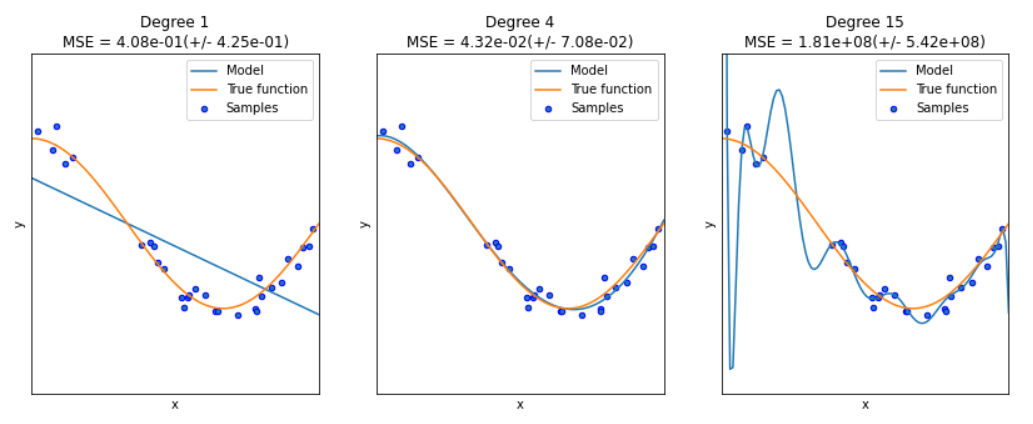
\includegraphics[width=\textwidth]{pictures/underfitting.png}
    
    We end up with the fundamental problem of overfitting/underfitting in ML. A lot of research is dedicated for general methods and special cases to efficently avoid overfitting/underfitting.
\end{frame}

\begin{frame}{Underfit, Overfit, Vanishing and Exploding Gradients}
    \begin{figure}
        \centering
        \begin{minipage}{0.5\textwidth}
            \centering
            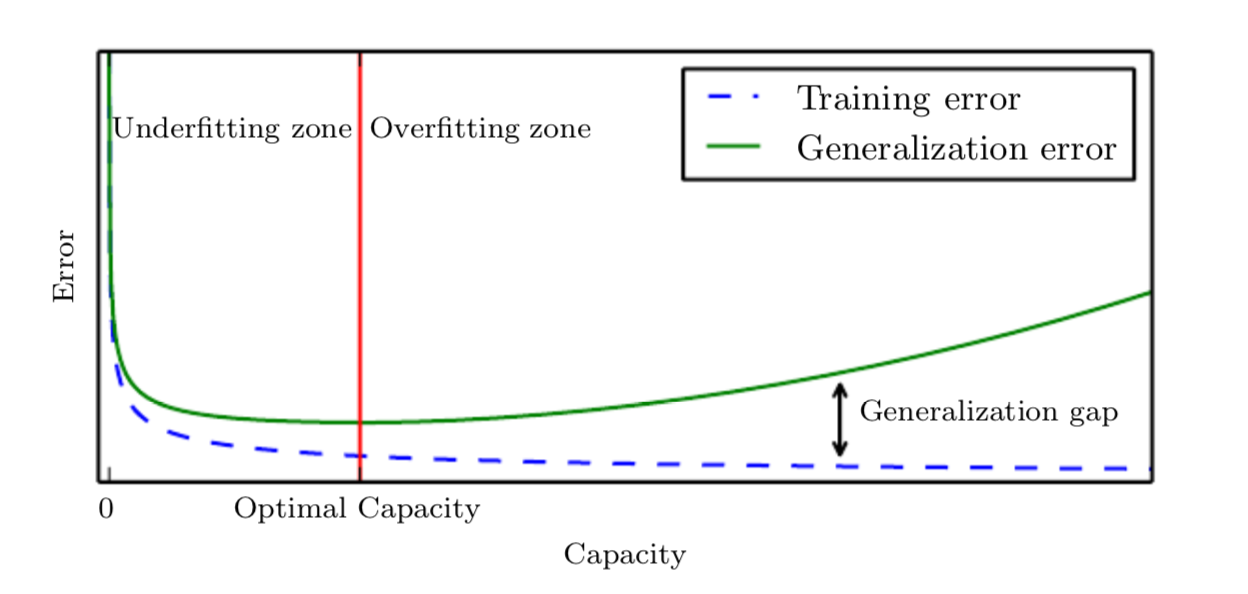
\includegraphics[width=\textwidth]{pictures/train_vs_validate.png}
            \caption{Fitting curve}
        \end{minipage}\hfill
        \begin{minipage}{0.5\textwidth}
            \centering
            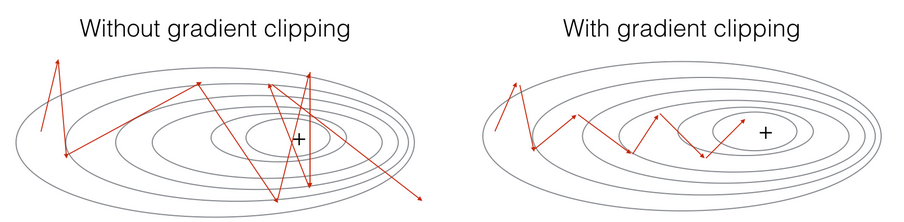
\includegraphics[width=\textwidth]{pictures/gradclip.png}
            \caption{Exploding gradient}
        \end{minipage}
    \end{figure}
    
    Apart from underfitting/overfitting problem, the most common one is vanishing/exploding gradients.\vspace{0.1in}
    
    When the objective function or optimization method was poorly selected, the gradient can take arbitrary big values or stay arbitrary small for long periods.
\end{frame}

\section{Decision Trees and Gradient Boosting}

\begin{frame}{Table of Contents}
    \tableofcontents[currentsection]
\end{frame}

\begin{frame}{Decision Trees - a simple classification algorithm}
    Consider the famous dataset - "Titanic passengers".\vspace{0.1in}
    
    Each object is a passenger.\vspace{0.1in}
    
    Features are: Ticket class, Sex, Age, \# of siblings / spouses, \# of parents / children, Ticket number, Passenger fare, Cabin number, Port of embarkation.\vspace{0.1in}
    
    Target is survival (0/1).\vspace{0.1in}
    
    How to solve this problem? Linear regression is definitely not the best approach.\vspace{0.1in}
    
    Idea: divide the data into parts based on very important features e.g. "Age", "Sex", and if some class is dominant in part, predict it for all objects from the part.\vspace{0.1in}
    
    Mathematically one can write split efficiency as combination of Variances/Entropy of target function at childs and root nodes.
\end{frame}

\begin{frame}{Decision Trees}
    \begin{center}
    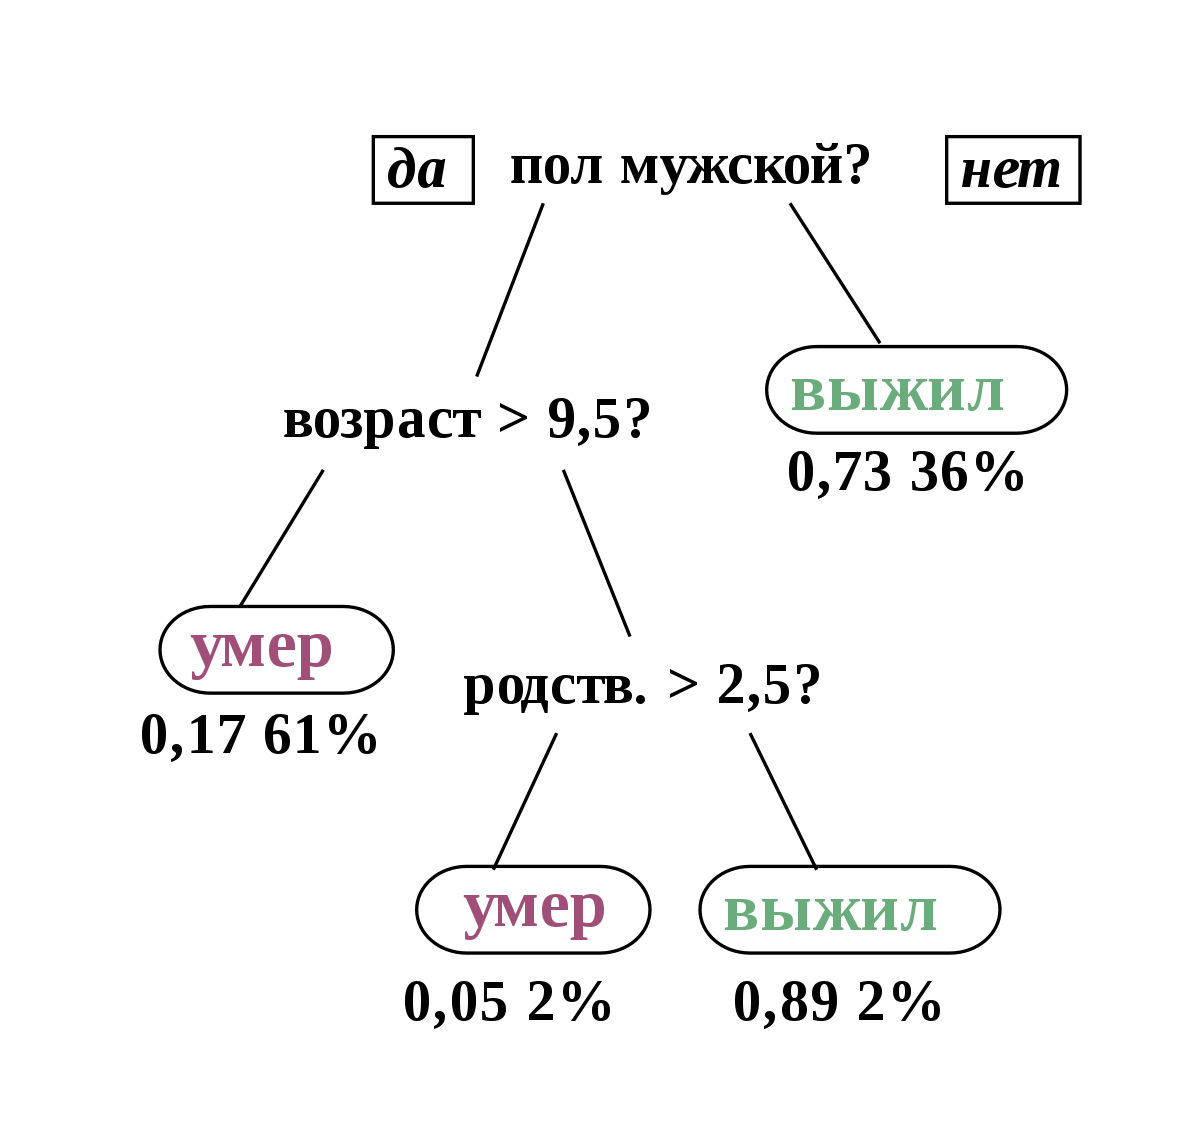
\includegraphics[width=0.7\textwidth]{pictures/titanic_decision_tree.png}
    \end{center}
\end{frame}

\begin{frame}{Gradient Boosting Decision Trees}
    Basic enhancement of Decision Tree Classifier is Random Forest Classifier - just generate many trees and average their prediction.\vspace{0.1in}
    
    Boosting is the following algorithm: train first model, subtract its prediction from the target, then train second model to predict the error produced by the first model and so on.\vspace{0.1in}
    
    Boosting on Decision Trees is a very strong baseline in many Classification and Regression problems: Credit scoring, House pricing, malicious bot traffic, CERN experiments, selling prediction(combination of time-series analysis and gradient boosting), customer uplift...\vspace{0.1in}
    
    Popular solutions: xgboost, LGBM(Microsoft), catboost(Yandex).
\end{frame}

\begin{frame}{Decision Trees + Random Forest + GBDT in code}
    \begin{center}
    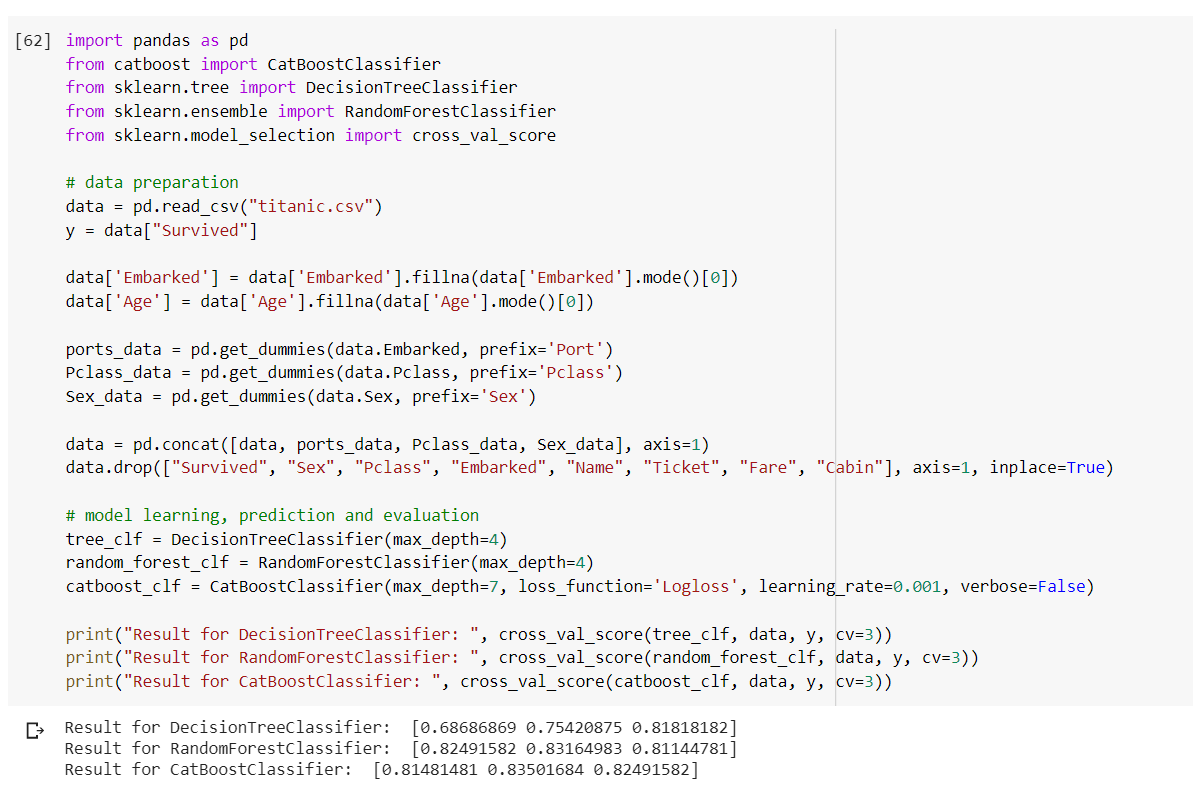
\includegraphics[width=\textwidth]{pictures/code_trees2.png}
    \end{center}
\end{frame}

\section{Neural Networks, CNN}

\begin{frame}{Table of Contents}
    \tableofcontents[currentsection]
\end{frame}

\begin{frame}{A Neural Network is...}
    a mathematical model for neural brain structure, based on old(1943) and wrong concept by neurophysiologist Warren McCulloch and genius mathematician Walter Pitts.\vspace{0.1in}
    
    For us it is directed acyclic graph (usually Layered) with Input Layer, Hidden Layers and Output Layer. 
    \begin{figure}
        \centering
        \begin{minipage}{0.5\textwidth}
            \centering
            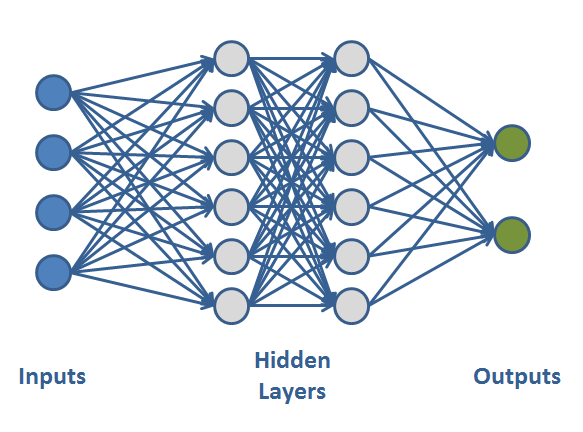
\includegraphics[width=\textwidth]{pictures/NN.png} % first figure itself
            \caption{Dense Layered Neural Network}
        \end{minipage}\hfill
        \begin{minipage}{0.5\textwidth}
            \centering
            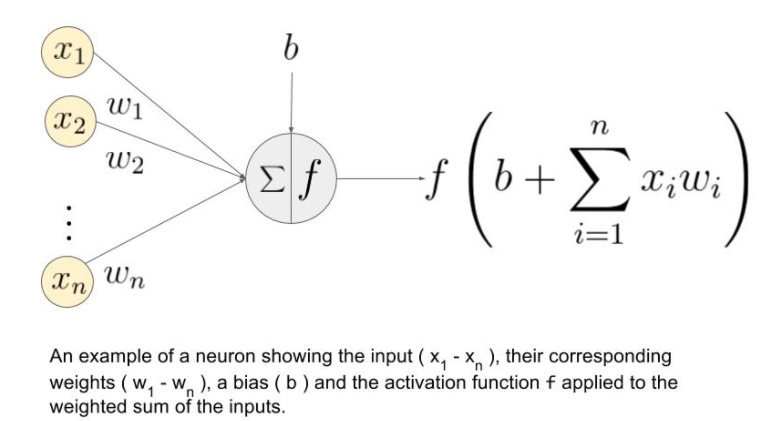
\includegraphics[width=\textwidth]{pictures/neuron.png} % second figure itself
            \caption{Neuron activation}
        \end{minipage}
    \end{figure}
\end{frame}

\begin{frame}{Computer Vision}
    Standard problems from Computer Vision include: 
    \begin{itemize}
        \item Classification e.g. recognize handwriting, ban inappropriate content.
        \item Object detection e.g. detect humans on the video in forbidden areas, detect forest fires / car traffic / new buildings  based on satellite images.
        \item Face recognition.
    \end{itemize}
    
    The common architecture is Convolutional Neural Network which, apart from usual layers, contains Convolutional Layers.
    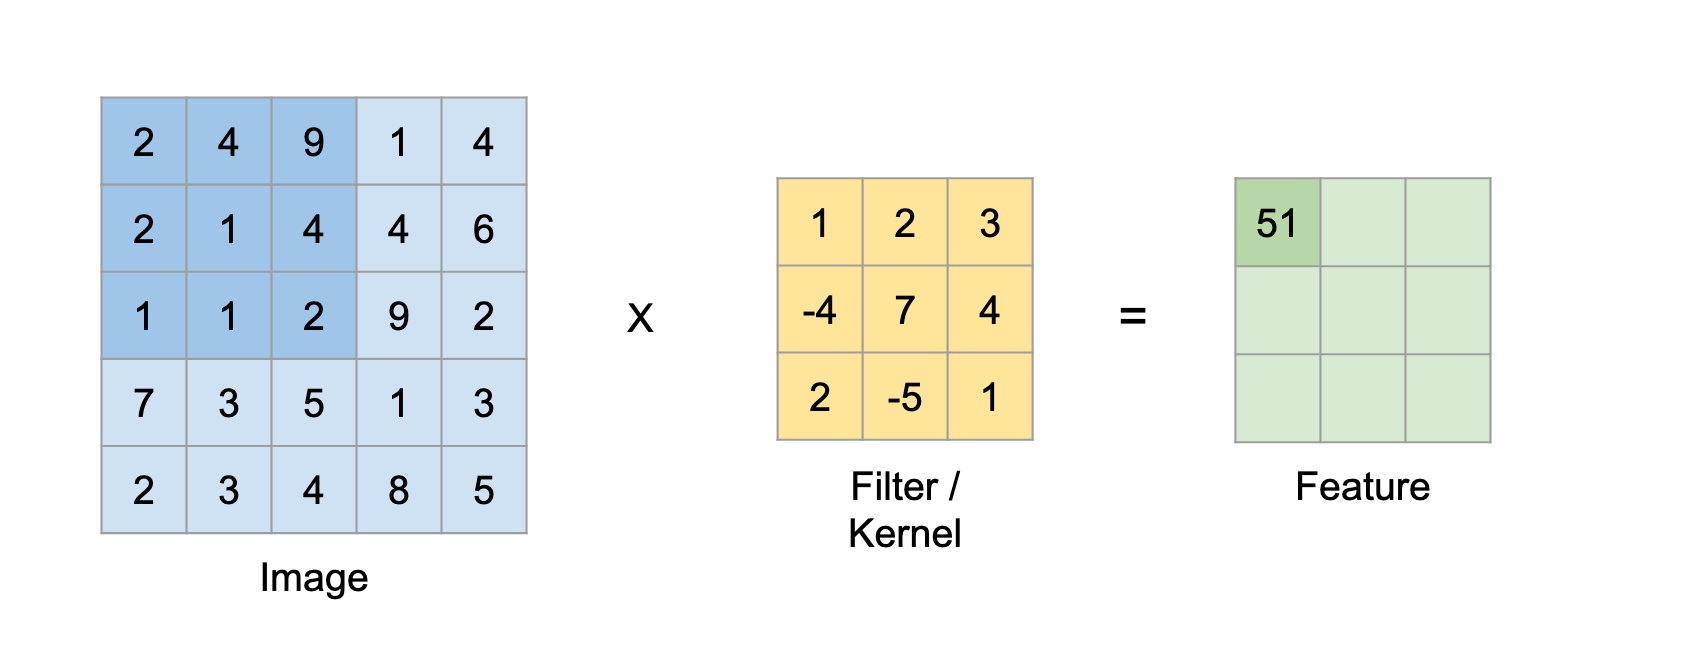
\includegraphics[width=0.9\textwidth]{pictures/convolution.png}
\end{frame}

\begin{frame}{Training Neural Networks}
    How to do gradient descent with 10 million dimensions and difficult intertwined objective? How to do a single step when the number of objects is hundreds of thousands or millions? How to handle overfitting/underfitting? How to handle vanishing/exploding gradients?\vspace{0.1in}
    
    \begin{itemize}
        \item Optimization is performed by batches (e.g. by sample of 256 images) otherwise one step would take too long.
        \item Gradient descent is done with special optimizers (Adam, RMSProp).
        \item The gradient is computed via special technique - backpropagation. Tensorflow and Pytorch are easy-to-use libraries for it.
        \item Activation function historically was the logistic curve, but due to vanishing gradients many others were tried. Currently mostly used are ReLU and LeakyReLU.
        \item To avoid overfitting, some neurons are randomly dropped from the learning scheme each step (Dropout layers). Other way to prevent overfitting is to use cropping/rotation/translation/scaling to generate more data.
    \end{itemize}
\end{frame}

\begin{frame}{Convolutional Neural Network Initialization code}
    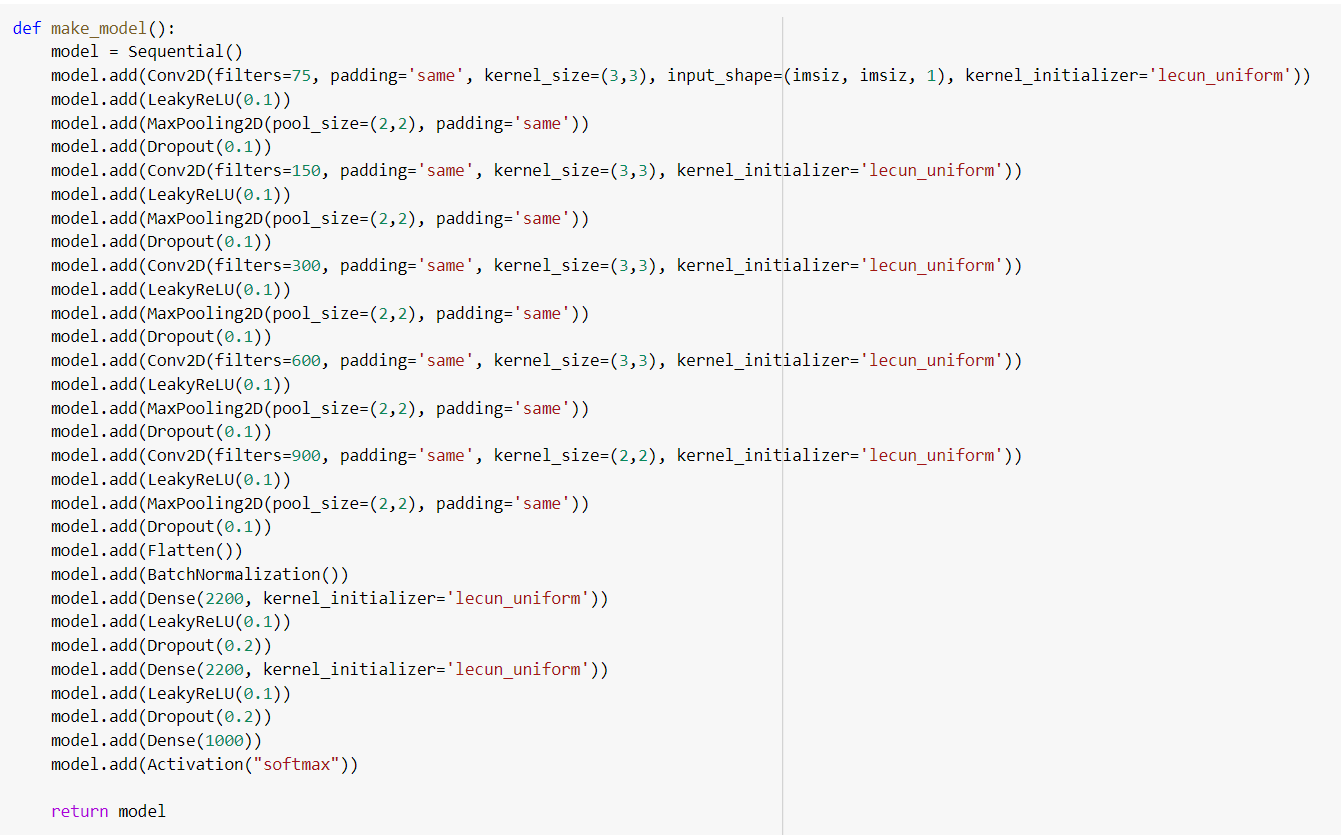
\includegraphics[width=\textwidth]{pictures/CNN_code.png}
\end{frame}

\begin{frame}{Chinese character recognition}
    This CNN is from one of our homework on recognition of 1000 different chinese characters. Full dataset contains millions of black and white $64\times 64$ images. Model has $\approx 2\cdot 10^7$ parameters and final accuracy of 98.07\%.\vspace{0.1in}
    
    Training on CPU takes $>8$ hours, on GPU it takes $\approx 40$ minutes. Google has invented special ASIC hardware TPU (Tensor Processing Unit) which allows to train huge Neural Networks within minutes.\vspace{0.1in}
    
    Remark: a program can be faster on GPU if its "bottleneck" is a simple operations as addition, or multiplication, or FFT, on a data that is 2 times larger than the CPU available memory limit.
\end{frame}

\begin{frame}{Remarks on Computer Vision}
    Deep Learning is a general term used describe Deep Neural Networks solutions. In CV Deep Learning is one of the ways to achieve State-of-the-Art classification results.\vspace{0.1in}
    
    In 2012 ImageNet competition one particular Deep CNN called AlexNet has beaten other models by more than 10\% in accuracy, this was the moment researchers and the industry started to pay much more attention to CV.\vspace{0.1in}
    
    Such models became much better than humans in image classification. And since ground truth is produced by humans, further research is focused on more difficult tasks such as segmentation or model compressing from millions of parameters to thousands thus making the inference faster.\vspace{0.1in}
    
    Right now (2020) the demand for CV ML Engineers and Research is overwhelming in the industry.
\end{frame}

\begin{frame}
    \begin{center}
    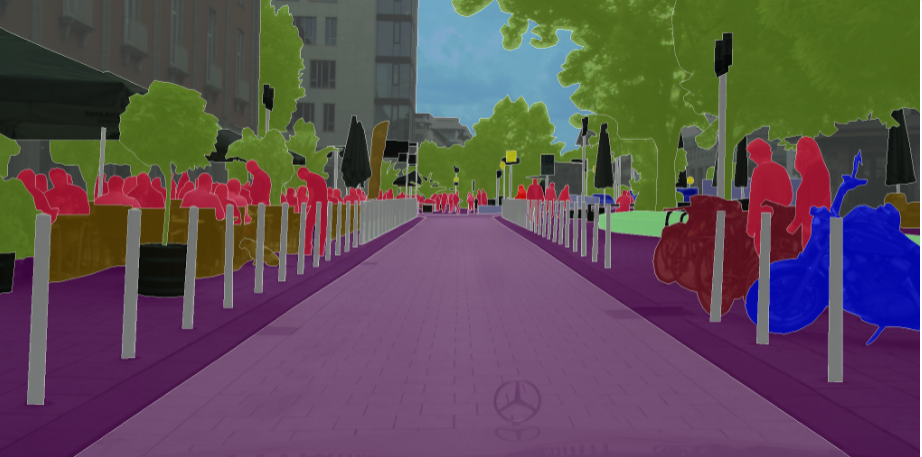
\includegraphics[width=\textwidth]{pictures/segmentation.png}
    \end{center}
\end{frame}

\section{Natural Language Processing}

\begin{frame}{Table of Contents}
    \tableofcontents[currentsection]
\end{frame}

\begin{frame}{Tasks in NLP}
    Wide range of applications:
    \begin{itemize}
        \item Text classification.
        \item Text translation, even multi-lingual translation is doable.
        \item Text generation.
        \item Document clusterization.
        \item Detection of simple bugs in code.
    \end{itemize}
    
    We always consider text as a sequence of letters or a sequence of words.\vspace{0.1in}
    
    First approaches were based on Markov chains with hidden parameters (1950s) and prediction of the next word in the text. They were too weak.
\end{frame}

\begin{frame}
    \frametitle{Simple solutions in NLP}
    Fast and simple solution of sufficient quality for Text classification and document clusterization can be produced by taking text to vector based on the word count (dimension is incredibly big!) and perform projection on a subspace of small dimension by SVM (Principal Component Analysis), then do linear regression.\vspace{0.1in}
    
    Another Interesting solution is Word2Vec - pre-trained embedding of English words into high-dimensional vector space with great behaviour. Close words are close vectors, and even some semantic relationships hold:
    
    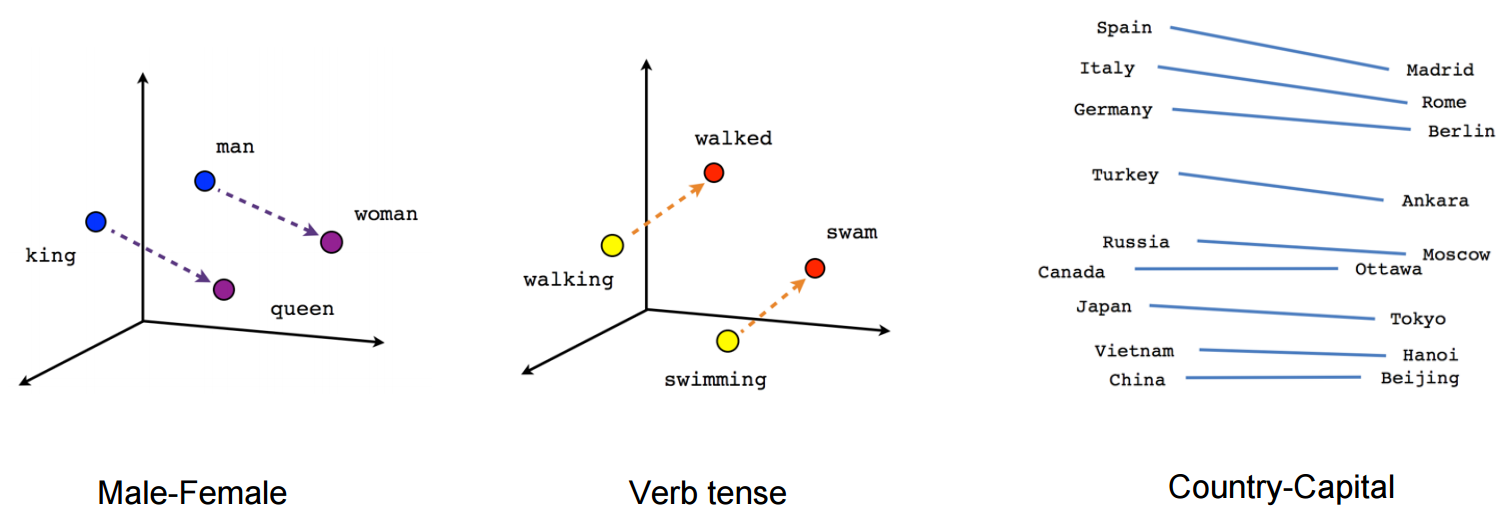
\includegraphics[width=\textwidth]{pictures/w2v.png}
\end{frame}

\begin{frame}
    \frametitle{State of the art solutions in NLP}
    First breakthroughs started with realization that large data allows generation of sentences by predicting the next \textit{character} instead of the next word.\vspace{0.1in}
    
    Recurrent Neural Networks (RNNs) and very similar models were dominating in the NLP a few years ago. Simplified description is the following:\vspace{0.1in}
    
    The model has a hidden state(vector in $\mathbb{R}^{N}$) which should "contain" information about current "context". With each new character the hidden state is adjusted and output is produced according to the last input and the current hidden state.
    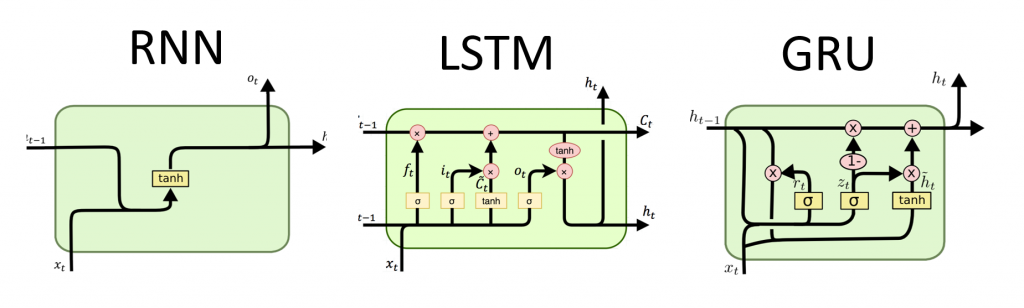
\includegraphics[width=0.8\textwidth]{pictures/lstm.png}
\end{frame}

\begin{frame}
    \frametitle{Transformers}
    Another major breakthrough was the paper \href{https://arxiv.org/abs/1706.03762}{"Attention Is All You Need"} (June 2017), where authors introduced "Transformer" architecture (Deep Neural Networks focused on Attention mechanism). This led to significant improvements of objectives in nearly all NLP tasks. Soon a variety of modifications like BERT and RoBERTa were produced.\vspace{0.1in}
    
    In June 2020 Generative Pre-trained Transformer 3 (GPT-3) was released by OpenAI. It has 175 billion parameters (human brain has 85-86 billion neurons on average). The training costed millions of dollars.\vspace{0.1in}
    
    Can do text summarization and answering questions. With small corrections by a human it can produce essays and articles on a variety of topics (indistinguishable from human). Capable of producing code for simple Python and Ruby tasks.\vspace{0.1in}
    
    Remark: one can use pre-trained BERT or GPT for his research or adjustment for his tasks.
\end{frame}

\section{Recommendation Systems}

\begin{frame}
    \frametitle{Table of Contents}
    \tableofcontents[currentsection]
\end{frame}

\begin{frame}{Problem formulation}
    Recommendation systems are used in Yandex, Spotify, Netflix, Amazon, Google.\vspace{0.1in}
    
    Given a set of users $U$, a set of items $I$ and some known results $r_{ui}$ with $(u,i) \in K$ - the interaction between user $u$ and item $i$ (for example, $r_{ui} = 1$ if user liked the movie and $-1$ if he disliked it, or $r_{ui} = \log_{2}(1 + N)$, where $N$ is the number of times user bought some item on Amazon), we wish to approximate $r_{ui}$ for the unseen pairs and do best recommendations for users.\vspace{0.1in}
    
    Solutions from simplest to hardest: average $r_{ui}$ along users and make constant prediction; K-Nearest Neighbours(Collaborative Filtering); Matrix Factorization; Factorization Machines.
\end{frame}

\begin{frame}{Simple solutions description}
    Fix $i$ and let $U'$ be the set of $(u,i) \in K$.\vspace{0.1in} 
    
    Constant prediction: Predict $\overline{r}_{ui} = \frac{1}{|U'|}\sum\limits_{r_{u'i}\in K}r_{u'i}$.\vspace{0.1in}
    
    K-Nearest Neighbours: 
    
    Consider users $u, u'$ as vectors in $\mathbb{R}^{|I|}$. 
    
    Normalize vectors: $\overline{u} = (r_{ui} - \overline{r}_{ui})_{i\in I}$ 
    
    Define metric between them as cosine metric between normalized vectors: $d(u, u') = \cos(\overline{u}, \overline{u}')$.
    
    Find K-Nearest Neighbours to the current vector and average their predictions.\vspace{0.1in}
    
    Matrix Factorization: Fix $k$. Suppose that $\exists v_i, v_u\in \mathbb{R}^{k}, i\in I, u\in U$ such that $r_{ui} = \langle v_u, v_i\rangle$. Learn $v_u, v_i$ via gradient descent(with appropriate reguralization). It is the same as learning matrix factorization $R = V_{U} \cdot V_{I}$.
\end{frame}

\begin{frame}{Factorization Machines}
    Factorization Machines is a generalization of Matrix Factorization. Suppose that apart from the $r_{ui}\in K$ we know some other user and item features, which is often the case. For example we know that user marked Rock as his favorite music genre, or that a song belongs to album from trendings.\vspace{0.1in}
    
    Let $x \in \mathbb{R}^d$ denote the vector and let us find the prediction $y$ as the second order polynomial regression: 
    $$y(x) = w_0 + \sum w_s\cdot x_s  + \sum w_{st}\cdot x_s x_t.$$
    
    The number of weights is $\frac{d^2 + d + 2}{2}$. Let us restrict to the case $w_{st} = \langle v_s, v_t\rangle$, where $v_s, v_t \in \mathbb{R}^r$. Then the number of weights becomes $rd + d + 1$. To recover FM model we should put $x_i, x_u = 1$ for user and item, then $$y(x) = w_0 + w_u + w_i + \langle v_u, v_i\rangle.$$
    Good Open Source realization: LightFM.
\end{frame}

\begin{frame}{Gradient descent}
    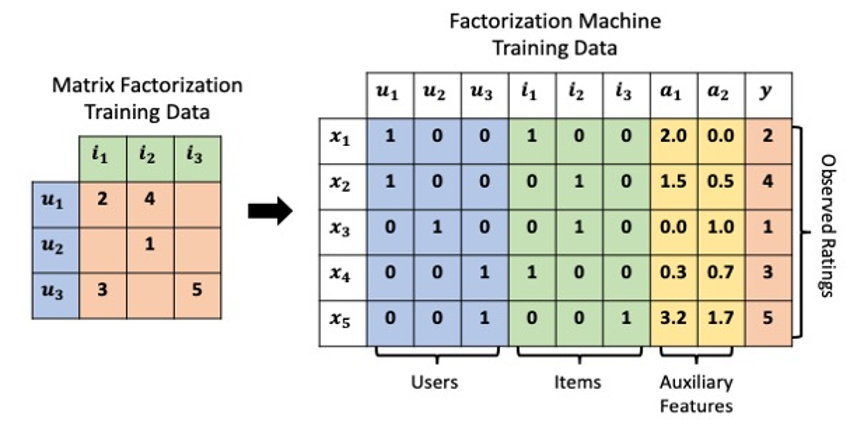
\includegraphics[width=0.85\textwidth]{pictures/recsysfm.png}
    
    Two most popular approaches to do optimization with Matrix Factorization are: 
    \begin{itemize}
        \item Stochastic Gradient Descent: batch optimization with batch size equal to 1.
        \item EM algorithm: Fix $V_{U}$, optimize $V_{I}$ by regression, then fix $V_{I}$, optimize $V_{U}$ and so on.
    \end{itemize}
\end{frame}

\section{Reinforcement Learning}

\begin{frame}{Table of Contents}
    \tableofcontents[currentsection]
\end{frame}

\begin{frame}
    RL is very challenging and very popular among researchers. General problem formulation is the following: we are given an \textbf{environment} (a game, a map) and an \textbf{agent} (computer bot playing a game or trying to navigate on the map). Each moment of time $t$ game is in some state $S_t$ and agent can perform \textbf{action} $A_t$ and for each his action we give him a reward $R(S_t, A_t)$.\vspace{0.1in}
    
    Mathematics behind: One way is to learn Markov chain probabilities of performing some action which maximizes the reward, namely, we learn a policy function
    $$\pi(a|s) = \mathbb{P}(A_t = a| S_t = s),$$
    to optimize the reward function
    $$\mathbb{E}_{\pi}(\sum\limits_{k = 0}^{\infty}\gamma^{k}R_{t+k+1}| S_t = s) .$$
    note that the sum is calculating the future rewards with an exponential decay $\gamma$. This way we can either try to learn immediate reward ($\gamma$ is small) or long-term rewards ($\gamma$ is close to $1$).
\end{frame}

\begin{frame}{Underfit/Overfit}
    As usual, we face the classical difficulties - underfitting and overfitting. In Reinforcement Learning both of these are still very challenging.
    
    Overfitting examples: 
    \begin{itemize}
        \item People tried to teach a car model to drive without crashes, the result was a car learning to drive backwards because this way crashes were not registered.
        \item Tetris bot learned to pause the game when he is in a definite losing position.
        \item Sometimes bots learn unexpected game behaviour unknown even to developers and experts.
    \end{itemize}
    
    Underfitting examples: 
    \begin{itemize}
        \item All the tasks mentioned on previous slides RL can't handle.
    \end{itemize}
\end{frame}

\begin{frame}{Games dominated by RL models}
    \begin{itemize}
        \item Chess
        \item Atari games dataset - humans still need less frames to learn, but SotA is close to beating us.
        \item Go - model description is available but it takes several millions of dollars to train.
        \item Dota - RL models have won against world champion team. 
        \item Starcraft - models lose to pro players if click speed is bounded and even if it is unbounded they still cannot beat best players. Note that the number of degrees of freedom is essentially infinite. The learning again costs millions of dollars.
    \end{itemize}
\end{frame}
\end{document} 